\section{PATH PLANNING}
\subsection{Robotic Operating System (ROS)}
% Figure Image =============================================================================
\begin{figure}[ht]
	\centering
	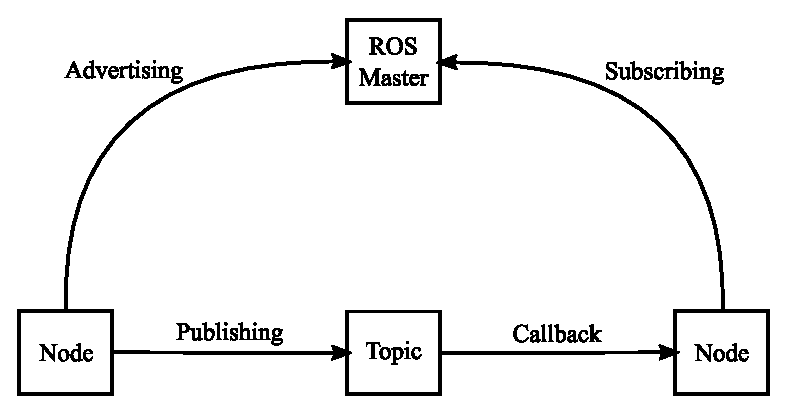
\includegraphics[scale=1]{images/imagess/6pp-ros.eps} 
	\caption{ROS Framework}
	\label{fig:ROS Framework}
\end{figure}
% Figure Image =============================================================================
\hspace{1.27cm}
Robotic operating system (ROS) is an open source framework developed for robotic purposes. It contains libraries and packages that are already built and ready to use for robots. ROS is a peer-to-peer network of processes that could run on multiple devices that are connected via network.(\cite{rosabout})\par
\hspace{1.27cm}
\textbf{\figureautorefname{ \ref{fig:ROS Framework}}}, ROS center of communication is ROS Master. ROS master acts as a keeper of topics and services, registration and information of ROS nodes. ROS nodes are the process of performing the computation. It publishes or subscribes ROS messages with other nodes via ROS topics. ROS message is a data that has been simplified into a structure.\par

\subsubsection{Odometry Message}
\hspace{1.27cm}
Odometry is the information of robot position and velocity within the environment. In 3D coordinate system, the robot position is represented as \([p_x\quad p_y\quad p_z]^T\) and the orientation of the robot is represented as roll, pitch, yaw in Euler angle representation. As our robot is in 2D planar motion, thus we only interested in \([p_x\quad p_y\quad \theta]^T\). When using the ROS message, the odometry directly publishes with the position and orientation of the robot from the simulated environment. The position is expressed as \([p_x\quad p_y]\) and the orientation in the quaternion form \((qw,qx,qy,qz)\).\par
\break
In this project the Odometry Message is used to contain the data of:
\begin{itemize}
	\item Lidar scan matching
	\item Wheel encoder odometry
	\item EKF fusion pose
	\item Robot true pose
	\item Robot current pose
\end{itemize}


% Table ====================================================================================
\begin{table}[ht]
    \begin{center}
		\caption{Odometry Properties (\cite{rosodom})}
		\label{Table: Odometry Properties}
		\begin{tabular}{p{0.4\linewidth}  p{0.5\linewidth}}
		ROS message & Definition \\
		\hline
        Header & Timestamp and frame id \\
        Child frame id &  \\
        Geometry\_msgs/PoseWithCovariance & Estimation of WMR Position in free space with uncertainty\\
        Geometry\_msgs/Pose & Contain the information of the position x,y,z and orientation in quaternion form (x,y,z,w)\\
        Geometry\_msgs/TwistWithCovariance & Estimation of WMR Velocity in free space with uncertainty \\
        Geometry\_msgs/Twist & Contain the information of velocity in linear and angular\\
        %\hline
        \ChangeRT{1.5pt} 
       \end{tabular}
  \end{center}
\end{table}

\textbf{\tableautorefname{ \ref{Table: Odometry Properties}}}, In the ROS Odometry properties, In global frame,\\
$\bullet$ \textbf{Robot poses is:}\par
\begin{itemize}
	\item Odometry.Pose.Pose.Position.x = \(p_x\)
	\item Odometry.Pose.Pose.Position.y = \(p_y\)
	\item Odometry.Pose.Pose.Orientation.(qw,qx,qy,qz) = \(\theta\)
\end{itemize}
$\bullet$ \textbf{Robot velocity is:}\par
\begin{itemize}
	\item Odometry.twist.twist.linear.x = \(\Dot{p_x}\)
	\item Odometry.twist.twist.linear.y = \(\Dot{p_y}\)
	\item Odometry.twist.twist.angular.z = \(\omega\)
\end{itemize}




\subsubsection{IMU Message}
\hspace{1.27cm}
IMU is a module that consists of three different types of sensors (triaxial). Those sensors are accelerometer, gyroscopes, and magnetometer, which measure the acceleration, the angular velocity, and the magnetic field, respectively. The IMU ROS message are used to show the data of velocity, acceleration, and orientation of a system in quaternion form.\par
\break
In this project the IMU Message is used to contain the data of:
\begin{itemize}
	\item Robot Estimated Orientation
	\item Robot linear and angular velocity
\end{itemize}

% Table ====================================================================================
\begin{table}[ht]
    \begin{center}
		\caption{IMU Properties (\cite{rosimu})}
		\label{Table: IMU Properties}
		\begin{tabular}{p{0.3\linewidth}  p{0.6\linewidth}}
		ROS message & Definition \\
		\hline
        Header & Timestamp and frame id \\
        Geometry\_msgs/Quaternion & Estimation of WMR orientation in quaternion form \\
        Geometry\_msgs/Vector3 & Contain the information of WMR angular velocity \\
        Geometry\_msgs/Vector3 & Contain the information of WMR linear acceleration \\
        %\hline
        \ChangeRT{1.5pt} 
       \end{tabular}
  \end{center}
\end{table}

\textbf{\tableautorefname{ \ref{Table: IMU Properties}}}, In the ROS IMU properties,\\
$\bullet$ \textbf{IMU data is:}\par
\begin{itemize}
	\item IMU.Orientation.(qw,qx,qy,qz) = \(\theta\)
	\item IMU.angular\_velocity = simulated angular velocity in (x,y,z)
	\item IMU.linear\_acceleration = simulated linear velocity in (x,y,z)
\end{itemize}






\subsubsection{Twist Message}
\hspace{1.27cm}
In ROS, twist is the message that carries the information of the velocity of the system in free space. The velocity of the system is decomposed into linear velocity and angular velocity. Furthermore the Twist message is used to publish the message for the mobile robot controller.\par

In this project the IMU Message is used to contain the data of:
\begin{itemize}
	\item Robot linear velocity along x-axis 
	\item Robot angular velocity about z-axis
\end{itemize}

% Table ====================================================================================
\begin{table}[ht]
    \begin{center}
		\caption{Twist Properties (\cite{rostwt})}
		\label{Table: Twist Properties}
		\begin{tabular}{p{0.3\linewidth}  p{0.6\linewidth}}
		ROS message & Definition \\
		\hline
        Geometry\_msgs/Vector3 & Contain the information of WMR linear velocity \\
        Geometry\_msgs/Vector3 & Contain the information of WMR angular velocity \\
        %\hline
        \ChangeRT{1.5pt} 
       \end{tabular}
  \end{center}
\end{table}

\textbf{\tableautorefname{ \ref{Table: Twist Properties}}}, In the ROS Twist properties, In local frame,\\
$\bullet$ \textbf{Robot velocity is:}\par
\begin{itemize}
	\item Twist.linear.x = \(V\)
	\item Twist.angular.z = \(\omega\)
\end{itemize}









\subsubsection{LIDAR Message}
\hspace{1.27cm}
Lidar is a remote sensing device that uses light pulses to detect the distance from an object and has been widely used for multipurposes including navigation and mapping. Lidar usually contains a laser scanner and DC motor. The DC motor rotates the laser scanner in a 360 degree circle to obtain a full 360 degrees of the environment. \textbf{\tableautorefname{ \ref{Table: Lidar Properties}}}\par
\hspace{1.27cm}
In the project, the Lidar data is used to create the occupancy grid map and robot localization in the sensor fusion section. Using the Scan Matching algorithm, the robot pose is measured and update in the EKF fusion.\par
% Table ====================================================================================
\begin{table}[ht]
    \begin{center}
		\caption{Lidar Properties (\cite{roslid})}
		\label{Table: Lidar Properties}
		\begin{tabular}{p{0.3\linewidth}  p{0.6\linewidth}}
		ROS message & Definition \\
		\hline
        header             & Timestamp and frame id \\
        angle\_min         & Started angle of scan \\
        angle\_max         & End angle of scan \\
        angle\_increment   & Angular distance between scan to scan \\
        time\_increment    & Time between one full scan to one full scan \\
        scan\_time         & Time between scan to scan \\
        range\_min         & Minimum range \\
        range\_max         & Maximum range \\
        ranges             & Range data in one full scan \\
        intensities        & Intensity data \\
        %\hline
        \ChangeRT{1.5pt} 
       \end{tabular}
  \end{center}
\end{table}















\subsubsection{Simulation, Visualization and Robot Model URDF}
\begin{figure}[ht]
	\centering
	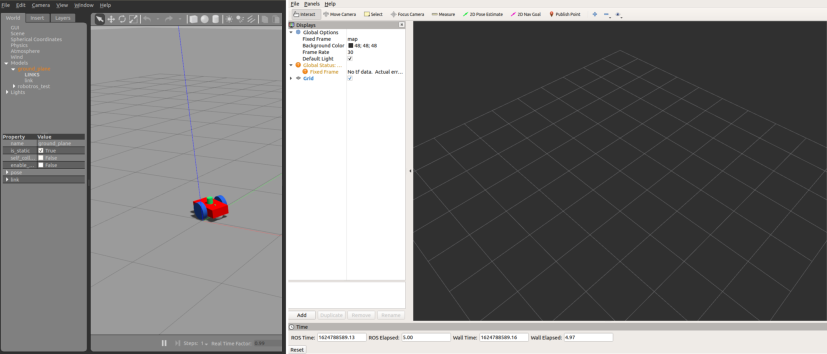
\includegraphics[scale=1]{images/imagess/6pp-rvgz.pdf}
%	\begin{tikzpicture}
%		\draw[step=1cm,gray,very thin] (0,0) grid (13,6);
%	\end{tikzpicture} 
	\caption{Gazebo and Rviz Window}
	\label{fig:Gazebo and Rviz Window}
\end{figure}
\hspace{1.27cm}
\textbf{\figureautorefname{ \ref{fig:Gazebo and Rviz Window}}}, the Gazebo robot simulation software will be used to simulate the robot, sensor and the surrounding environment. The RVIZ is used as a visualization tool. RVIZ allows us to visualize and verify the incoming data from the ROS messages. In this project, RVIZ is used to visualize the Occupancy Grid Map, Robot Model, Robot trajectory -etc.\par












\subsection{Path Planning A*}
\hspace{1.27cm}
A* algorithm is one of the path search algorithm that is widely used in many fields. In the mobile robotic field, the algorithm is used for searching the path in a robot navigation task. In this project, the A* algorithm is used to search the path for the mobile robot. The information that is given to the algorithm are the start point (robot current position), goal point (desired point to move to), and the occupancy grid map (which contain the free space and the occupied space of the environment).





















\subsubsection{Occupancy Grid Map}
\hspace{1.27cm}
Occupancy grid map is one of many pieces of information that are required for the mobile robot for navigation tasks such as path planning, navigation, environment map, and localization.\par
\hspace{1.27cm}
Occupancy grid map represents the environment in square grid cells. Each of grid cells is represented as either an occupied cell or a free cell according to the calculation of the binary probability value. \textbf{\figureautorefname{ \ref{fig:Occupancy Grid Map}}}, Occupancy Grid Map is a 2D map is a large set that contains a probability value in every cell. The cell representation as:
\begin{itemize}
	\item \textbf{Occupied cell} by probability value of (1) with black color
	\item \textbf{Free cell} by a probability value of (0) with white color
\end{itemize}
With the assumption of that the cell is either occupied or free, each probability value contained in each cell are independent, and the surrounding environment is static. Occupancy grid maps are fine-grained grids defined over the continuous space of locations and often used after solving the SLAM problem by some other means and taking the resulting path estimates for granted. \textbf{\tableautorefname{ \ref{Table: Occupancy Grid Map Properties}}} is ROS properties of Occupancy Grid Map.\par

\begin{figure}[ht]
	\centering
	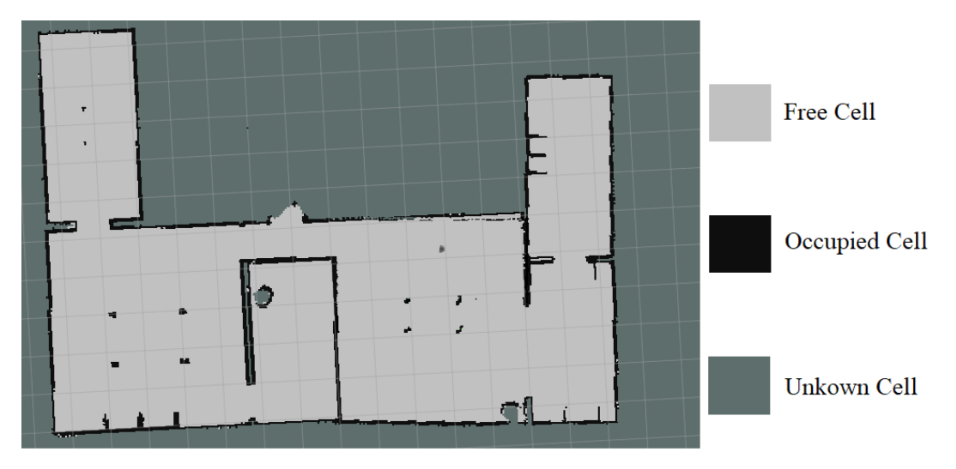
\includegraphics[scale=1]{images/imagess/6pp-pathplan_ogm.eps} 
	\caption{Occupancy Grid Map}
	\label{fig:Occupancy Grid Map}
\end{figure}
% Figure Image =============================================================================

% Table ====================================================================================
\begin{table}[ht]
    \begin{center}
		\caption{Occupancy Grid Map Properties (\cite{rosocm})}
		\label{Table: Occupancy Grid Map Properties}
		\begin{tabular}{p{0.3\linewidth}  p{0.6\linewidth}}
		ROS message & Definition \\
		\hline
        header                   & Timestamp and frame id \\
        nav\_msgs/MapMetaData    & Contain the map's resolution (m/cell), width (cell), height (cell) and origin (0,0) \\
        int8[] data              & Contain the array of probability value of map \\
        %\hline
        \ChangeRT{1.5pt} 
       \end{tabular}
  \end{center}
\end{table}
% Table ====================================================================================


\break
\hspace{1.27cm}
\textbf{\figureautorefname{ \ref{fig:Occupancy Grid Map Cell Value}}}, SLAM start with the initialization of an empty cell grid. Each cell has an address in the grid and its size is determined by the algorithm or user assign value. Then, the empty grid is filled with probability value to represent the obstacle in the environment where the robot can not traverse on.\par
\begin{figure}[ht]
	\centering
	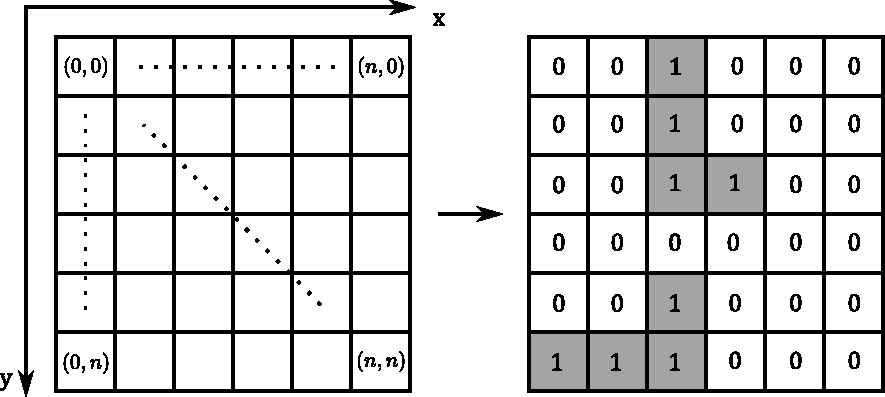
\includegraphics[scale=1]{images/imagess/6pp-ocm-cell-value.pdf}
%	\begin{tikzpicture}
%		\draw[step=1cm,gray,very thin] (0,0) grid (6,6);
%		\draw[step=1cm,gray,very thin] (7,0) grid (13,6);
%	\end{tikzpicture} 
	\caption{Occupancy Grid Map Cell Value}
	\label{fig:Occupancy Grid Map Cell Value}
\end{figure}










\subsubsection{A* Algorithm}
\hspace{1.27cm}
A* algorithm is an algorithm that based on the heuristic method. A* is the optimal best-first search algorithm. A* calculates the travel cost to the neighbor node from the current node. Node with the lowest cost to travel to is chosen.\par
The cost function is:
\begin{equation}
F(n)=G(n)+H(n)
\end{equation}

Where:
\begin{itemize}
	\item {\makebox[1cm]{\(F(n)\)\hfill} is the total cost of node path}
	\item {\makebox[1cm]{\(G(n)\)\hfill} is the exact distance from the starting node to the current node}
	\item {\makebox[1cm]{\(H(n)\)\hfill} is the estimation distance from the current node to the ending node}
	\item {\makebox[1cm]{\(n\)\hfill} is the node}

%	\item \(F(n)\) is the total cost of node path
%	\item \(G(n)\) is the exact distance from the starting node to the current node
%	\item \(H(n)\) is the estimation distance from the current node to the ending node. (Heuristic part of the cost function, meaning it is a guess)
%	\item \(n\) is the node
\end{itemize}

\hspace{1.27cm}
From SLAM, we obtain the occupancy grid like in figure shown below. \textbf{\figureautorefname{ \ref{fig:Occupancy Grid Map Example}}}, Each cell in the grid have its own address and the occupied value depending on SLAM. Let the origin address of the grid be in the top left corner, same as the occupancy grid map SLAM.\par
\begin{figure}[ht]
	\centering
	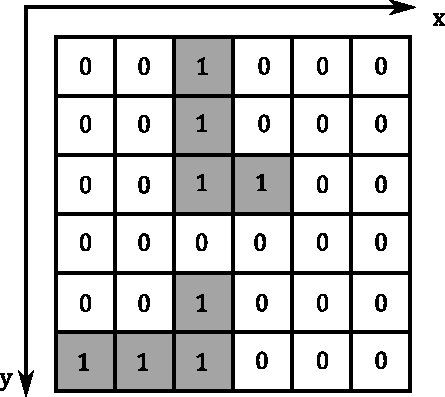
\includegraphics[scale=1]{images/imagess/6pp-ocm-cell-exmpl.pdf}
%	\begin{tikzpicture}
%		\draw[step=1cm,gray,very thin] (0,0) grid (6,6);
%	\end{tikzpicture} 
	\caption{Occupancy Grid Map Example}
	\label{fig:Occupancy Grid Map Example}
\end{figure}


\hspace{1.27cm}
\textbf{\figureautorefname{ \ref{fig:Astar starting point and ending point}}}, The white cell represents the space where the robot can move and the black cell represents the space where the robot can not move. Which mean, the starting point and the ending point have to be on chosen on the white cell address.\par
\begin{figure}[ht]
	\centering
	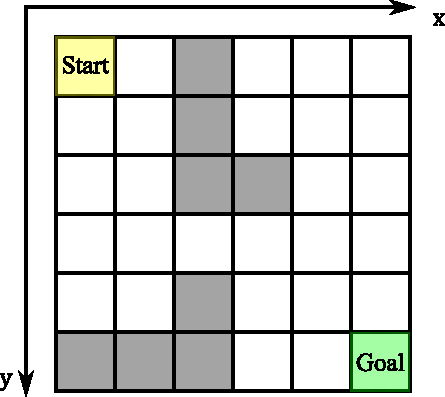
\includegraphics[scale=1]{images/imagess/6pp-ocm-start-goal.pdf}
%	\begin{tikzpicture}
%		\draw[step=1cm,gray,very thin] (0,0) grid (6,6);
%	\end{tikzpicture} 
	\caption{Astar starting point and ending point}
	\label{fig:Astar starting point and ending point}
\end{figure}


In A* cell, the cell contain 4 information, which are:
\begin{itemize}
	\item Address
	\item \(F\) value
	\item \(G\) value
	\item \(H\) value
\end{itemize}
\break
$\bullet$ \textbf{$G(n)$ value}\par
\hspace{1.27cm}
In \textbf{\figureautorefname{ \ref{fig:Euclidean Distance of G value}}}, to calculate the value of \(G(n)\) the exact distance from the starting point to the current node, we can use the Euclidean distance formula:\par

\begin{figure}[ht]
	\centering
	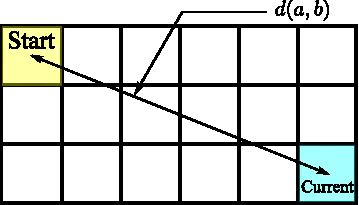
\includegraphics[scale=1]{images/imagess/6pp-eud-g.pdf}
%	\begin{tikzpicture}
%		\draw[step=1cm,gray,very thin] (0,0) grid (6,3);
%	\end{tikzpicture} 
	\caption{Euclidean Distance of G value}
	\label{fig:Euclidean Distance of G value}
\end{figure}
\begin{equation}
	d(a,b)^2 = (x_b - x_a)^2 + (y_b - y_a)^2
\end{equation}
\begin{equation}\label{eq:PP_euclidean_dis}
	d(a,b) = \sqrt{(x_b - x_a)^2 + (y_b - y_a)^2}
\end{equation}
Where:
\begin{itemize}
	\item {\makebox[2cm]{\(d(a,b)\)\hfill} is the distance from point a to point b}
	\item {\makebox[2cm]{\(x_a\), \(x_b\)\hfill} are the cell address of a and b in x-axis}
	\item {\makebox[2cm]{\(y_a\), \(y_b\)\hfill} are the cell address of a and b in y-axis}
	
%	\item \(d(a,b)\) is the distance from point a to point b
%	\item \(x_a\) and \(x_b\) is the cell address of a and b in x-axis
%	\item \(y_a\) and \(y_b\) is the cell address of a and b in y-axis
\end{itemize}

\break
$\bullet$ \textbf{$H(n)$ value}\par
\hspace{1.27cm}
In \textbf{\figureautorefname{ \ref{fig:Euclidean Distance of H value}}}, to calculate the value of \(H(n)\) the estimation distance from the current node to the ending node, we can use the Euclidean distance formula same as the \ref{eq:PP_euclidean_dis}. The value \(H(n)\) is the Heuristic part of the cost function, meaning it can be a guess value. Thus, in coding the square root can be dropped for the performance optimization.\par

\begin{figure}[ht]
	\centering
	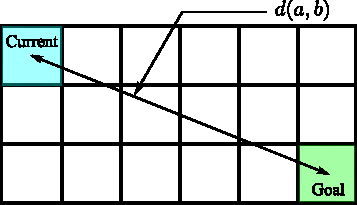
\includegraphics[scale=1]{images/imagess/6pp-eud-h.pdf}
%	\begin{tikzpicture}
%		\draw[step=1cm,gray,very thin] (0,0) grid (6,3);
%	\end{tikzpicture} 
	\caption{Euclidean Distance of H value}
	\label{fig:Euclidean Distance of H value}
\end{figure}


$\bullet$ \textbf{Parent and Child Cell} \par
\hspace{1.27cm}
In \textbf{\figureautorefname{ \ref{fig:Parent and Child Cell}}}, each cell has child cell and parent cell. Parent cell is a cell where the current node state is land on. The Child cell is the 8 neighbor cells around the parent cell.\par

\begin{figure}[ht]
	\centering
	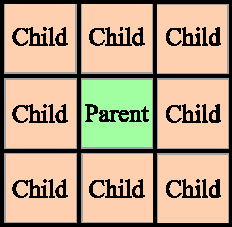
\includegraphics[scale=1]{images/imagess/6pp-par-chld.pdf}
%	\begin{tikzpicture}
%		\draw[step=1cm,gray,very thin] (0,0) grid (3,3);
%	\end{tikzpicture} 
	\caption{Parent and Child Cell}
	\label{fig:Parent and Child Cell}
\end{figure}

$\bullet$ \textbf{Initialize} \par
\hspace{1.27cm}
At start, the current node state is set to the start cell. The $H(n)$ and $G(n)$ of the cell is calculated using the \ref{eq:PP_euclidean_dis}. The $F(n)$ is the sum of the $G(n)$ and $H(n)$ \textbf{\figureautorefname{ \ref{fig:Start Point F,G,H}}}. Create 2 lists: Open list and Closed List.\par

\begin{itemize}
	\item Open List contains the cell which the cost value is yet to be calculated or traversed pass.
	\item Closed List contains the cell which the cost value is calculated or traversed pass or block by the obstacle.
\end{itemize}

Starting by adding the start cell to the Open List. After calculate the cost value, move it to the Closed List.

\break
\begin{figure}[ht]
	\centering
	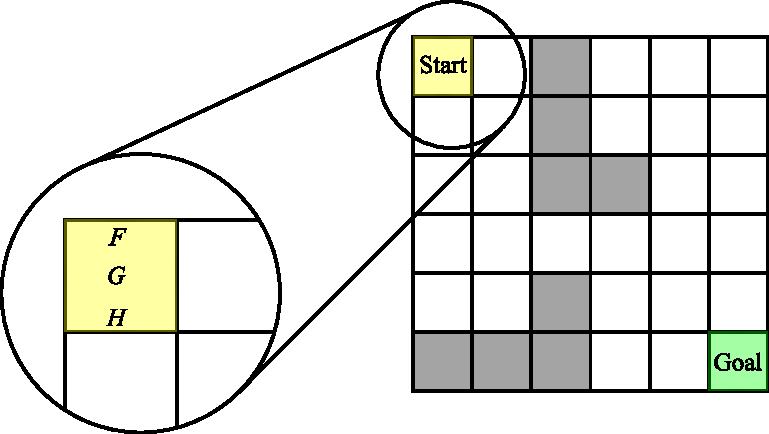
\includegraphics[scale=0.85]{images/imagess/6pp-start-cost.pdf}
%	\begin{tikzpicture}
%		\draw[step=1cm,gray,very thin] (0,0) grid (6,6);
%	\end{tikzpicture} 
	\caption{Start Point $F(n),G(n),H(n)$}
	\label{fig:Start Point F,G,H}
\end{figure}

$\bullet$ \textbf{Current state transition} \par
\hspace{1.27cm}
The $F(n),G(n),H(n)$ of the child cell to the parent cell is calculated (ignore the block cell) and add those to the Open List. If the $F(n)$ value of the child cell is the smallest of every cell, the current cell state is transit to that child cell, and it becomes the parent cell to the other. This action is loop until the goal point is found (the goal point is added to the Closed List). Then, backtracking the path from the goal to start as shown in \textbf{\figureautorefname{ \ref{fig:Current state transition}}}.\par

\begin{figure}[ht]
	\centering
	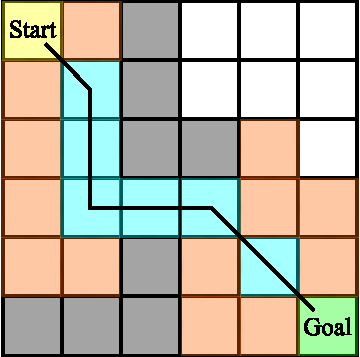
\includegraphics[scale=0.85]{images/imagess/6pp-transistion.pdf}
%	\begin{tikzpicture}
%		\draw[step=1cm,gray,very thin] (0,0) grid (6,6);
%	\end{tikzpicture} 
	\caption{Current state transition}
	\label{fig:Current state transition}
\end{figure}


$\bullet$ \textbf{A* pseudo-code} \par

\textbf{\tableautorefname{ \ref{Table: A* Pseudo-code}}} shows the pseudo-code for the A* algorithm. \textbf{\figureautorefname{ \ref{fig:A* Flowchart}}} shows the flowchart of the A* algorithm. Input data for the algorithm are: Occupancy Grid Map, Start node and Goal node. Output data for the algorithm is Pathway.







\begin{table}[ht]
	\caption{A* Pseudo-code}
	\label{Table: A* Pseudo-code}
	\begin{algorithm}[H]
	\SetAlgoLined
	\KwData{Occupancy Grid Map, Start, Goal}
	\KwResult{Path}
	INITIALIZE\;
	Let the $openList$ equal empty list of nodes\;
	Let the $closedList$ equal empty list of nodes\;
	Put the $startNode$ on the $openList$ (leave it's $f$ at zero)\;
	\While{the $openList$ is not empty}{
		Let the $currentNode$ equal the node with the least $f$ value\;
		Remove the $currentNode$ from the $openList$\;
		Add the $currentNode$ to the $closedList$\;
		\If{$currentNode$ is the goal}{
			Path Found. Backtraking to the start\;
		}
		Let the children of the $currentNode$ equal the adjacent nodes\;
		\For{each child in the children}{
			\If{child is in the $closedList$}{continue to beginning of for loop}
			$child.g$ = $currentNode.g$ + distance between child and current\;
			$child.h$ = distance from child to end\;
			$child.f$ = $child.g$ + $child.h$\;
			\If{$child.position$ is in the $openList$'s nodes positions}{\If{the $child.g$ is higher than the $openList$ node's $g$}{continue to beginning of for loop}
			Add the child to the openList}
		}
	}
	\caption{A* Pseudo-code (\cite{nicholasswift})}
	\end{algorithm}
\end{table}

\begin{figure}[ht]
	\centering
	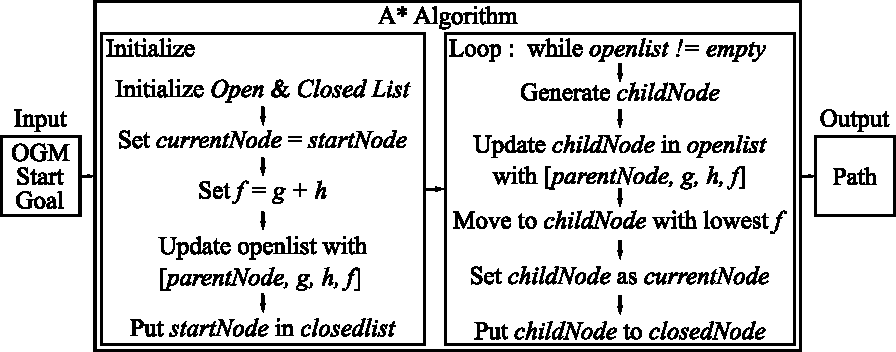
\includegraphics[scale=1]{images/imagess/6pp-astarfc.pdf}
	\caption{A* Flowchart}
	\label{fig:A* Flowchart}
\end{figure}